\chapter{Test}
Il sistema è stato testato sul ``Prontuario muto per l'esame orale"\cite{Prontuario}, un eserciziario con esempi e soluzioni di vari quiz utile per chi vuole la patente. La sezione che soddisfa gli obiettivi del progetto è ``Precedenze" che elenca 66 incroci corredati da soluzioni alla fine. Di questi, vengono tralasciati gli ultimi 8 perché non ci sono le informazioni relative al verso della manovra dei veicoli (dritto, destra o sinistra), rimanendo infine con 58 incroci da risolvere. Essi sono stati formalizzati e memorizzati nella base di conoscenza \texttt{kb.pl}, ognuno in un oggetto \texttt{incrocio/2}, con un ID e la lista dei fatti che descrivono l'incrocio come argomenti.

Per avviare il test viene usato il predicato \texttt{test/0} del modulo \texttt{main.pl} così definito:


\begin{verbatimtab}
test :-
	findall(ID, incrocio(ID, _), IDs),
	soluzione(IDs).
\end{verbatimtab}

\noindent
Mentre \texttt{soluzione/1} si presenta come:
\begin{verbatimtab}
soluzione([ID | T]) :-
	writeln(ID),
	pulisci,
	recupera_incrocio(ID, _),
	menu_utente:risolvi,
	soluzione(T).

soluzione([]).
\end{verbatimtab}

Vengono ritrovati tutti gli ID che servono a caricare gli incroci, poi risolti ad uno ad uno. Il comando da lanciare da riga di comando è:
\begin{verbatimtab}
swipl -f main.pl -t test > soluzioni
\end{verbatimtab}

\noindent
L'output viene raccolto in un file \texttt{soluzioni}, che si presenta così:
\scriptsize\verbatiminput{soluzioni}

\normalsize
Di seguito viene mostrata la soluzione del prontuario:

\newgeometry{top=.5cm,bottom=.5cm}
\begin{figure}[htbp!]
	\thisfloatpagestyle{empty}
	\centering
	\makebox[\linewidth][c]{
		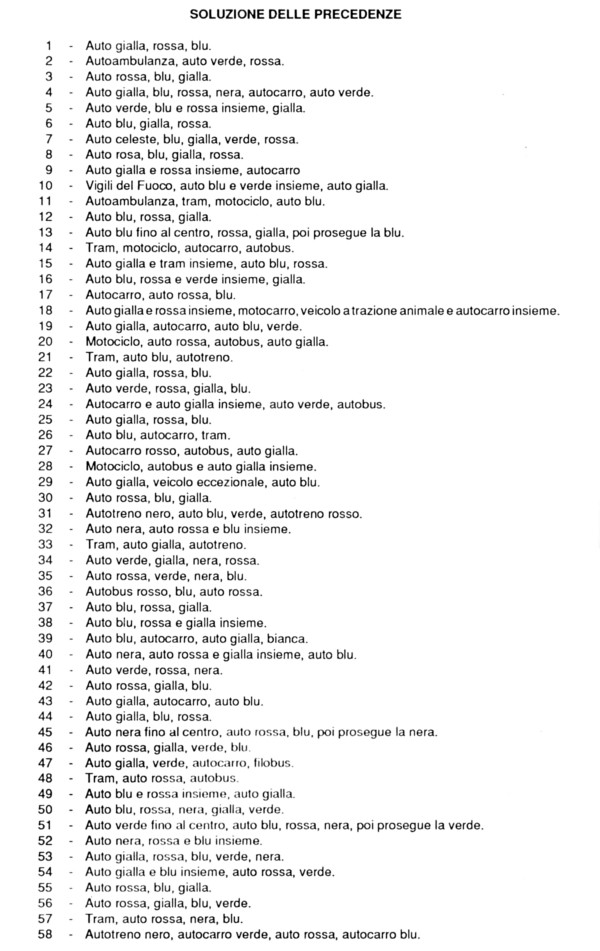
\includegraphics[width=1.25\textwidth]{images/sol}
	}
	\label{fig:sol}
\end{figure}

\restoregeometry

Prestando attenzione, si nota che gli incroci, la cui soluzione è discordante da quella fornita dal sistema, sono il n. 15 e il n. 26:
\begin{figure}[htbp!]
	\centering
	\begin{subfigure}[b]{.4\textwidth}
		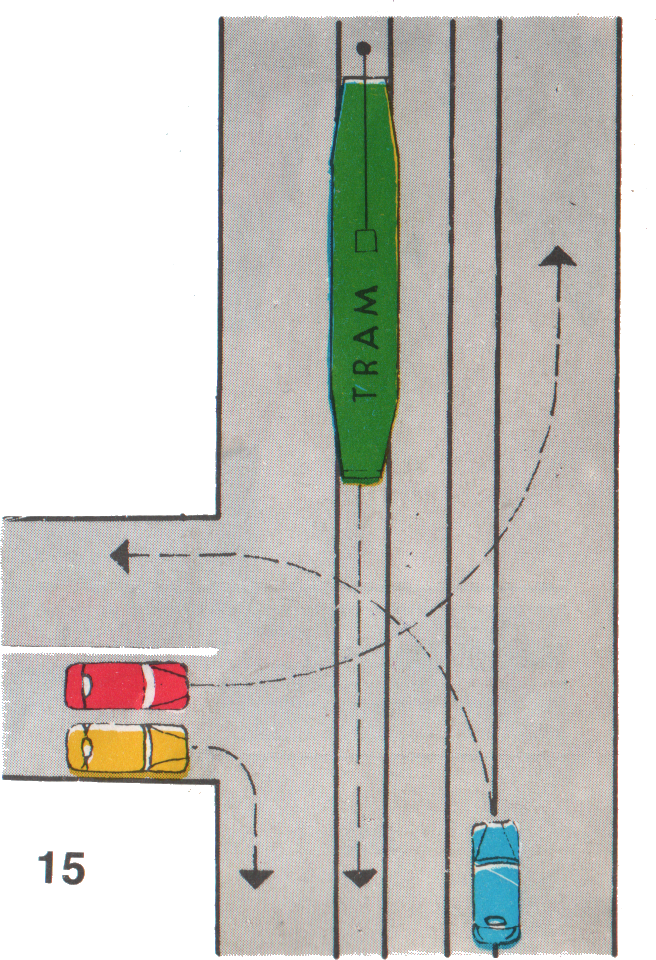
\includegraphics[width=\textwidth]{./images/fig15}
		\caption{Incrocio 15}
		\label{fig:15}
	\end{subfigure}
	\begin{subfigure}[b]{.4\textwidth}
		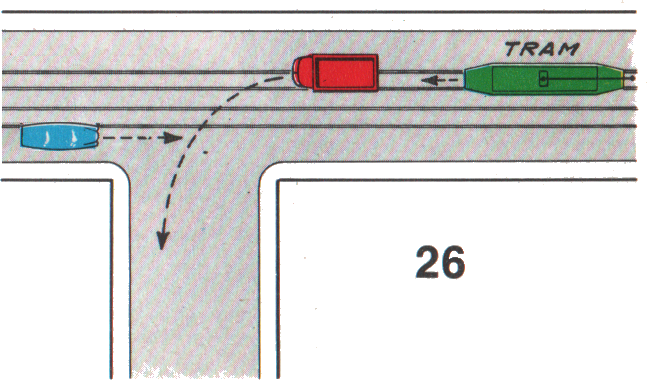
\includegraphics[width=\textwidth]{./images/fig26}
		\caption{Incrocio 26}
		\label{fig:26}
	\end{subfigure}
	\caption{Casi non conformi}
	\label{fig:disc}
\end{figure}



\begin{center}
	\begin{tabularx}{\textwidth}{cXXX}
		\hline
		\textbf{Incrocio} & \multicolumn{1}{c}{\textbf{Sistema}} & \multicolumn{1}{c}{\textbf{Prontuario}} & \multicolumn{1}{c}{\textbf{Spiegazione}} \\ \hline
		\adjustbox{raise=-1.4cm}{15} & 	\textit{Il veicolo tram è il primo a passare; 
					I veicoli blu, giallo passano insieme;
					Il veicolo rosso è l'ultimo a passare;} & \textit{Auto gialla e tram insieme, auto blu, rossa} & Il tram è prioritario, quindi passa per primo rispetto agli altri. Bisogna trattare il concetto di corsia, o di rotaie su strada.  \\ \hline
		\adjustbox{raise=-1.3cm}{26} & 	\textit{Il veicolo tram è il primo a passare;
				Il veicolo blu è il prossimo a passare;
				Il veicolo rosso è l'ultimo a passare;} & \textit{Auto blu, autocarro, tram} & Stesso motivo, il tram è prioritario. Bisogna trattare il concetto di coda tra veicoli. \\ \hline
	\end{tabularx}
\end{center}
